\documentclass{article}
\usepackage[round]{natbib}
\usepackage{graphicx}
\usepackage{amsmath}
\usepackage{amsfonts}
\usepackage{amssymb} 

\bibliographystyle{plainnat}

\newcommand{\cN}{\mathcal{N}}
\newcommand{\R}{\mathbb{R}}
\newcommand{\bX}{\mathbf{X}}
\DeclareMathOperator*{\argmin}{arg\,min}
\DeclareMathOperator*{\diag}{diag}

\title{Comparison of structured regularized SVD\\ and factor analysis}
\author{Lukasz, Trevor}
\begin{document}
\maketitle

%% \section*{Plan}

%% \begin{enumerate}
%%   \item Show that reduced-rank SVD approximates factor model
%%   \item Sparse reduced-rank rank
%% \end{enumerate}

\section{Motivation}

Given spase observations of a process in multiple individuals, can we recover individual trajectories (Fig. \ref{fig:motivation})?

\begin{figure}[h]
  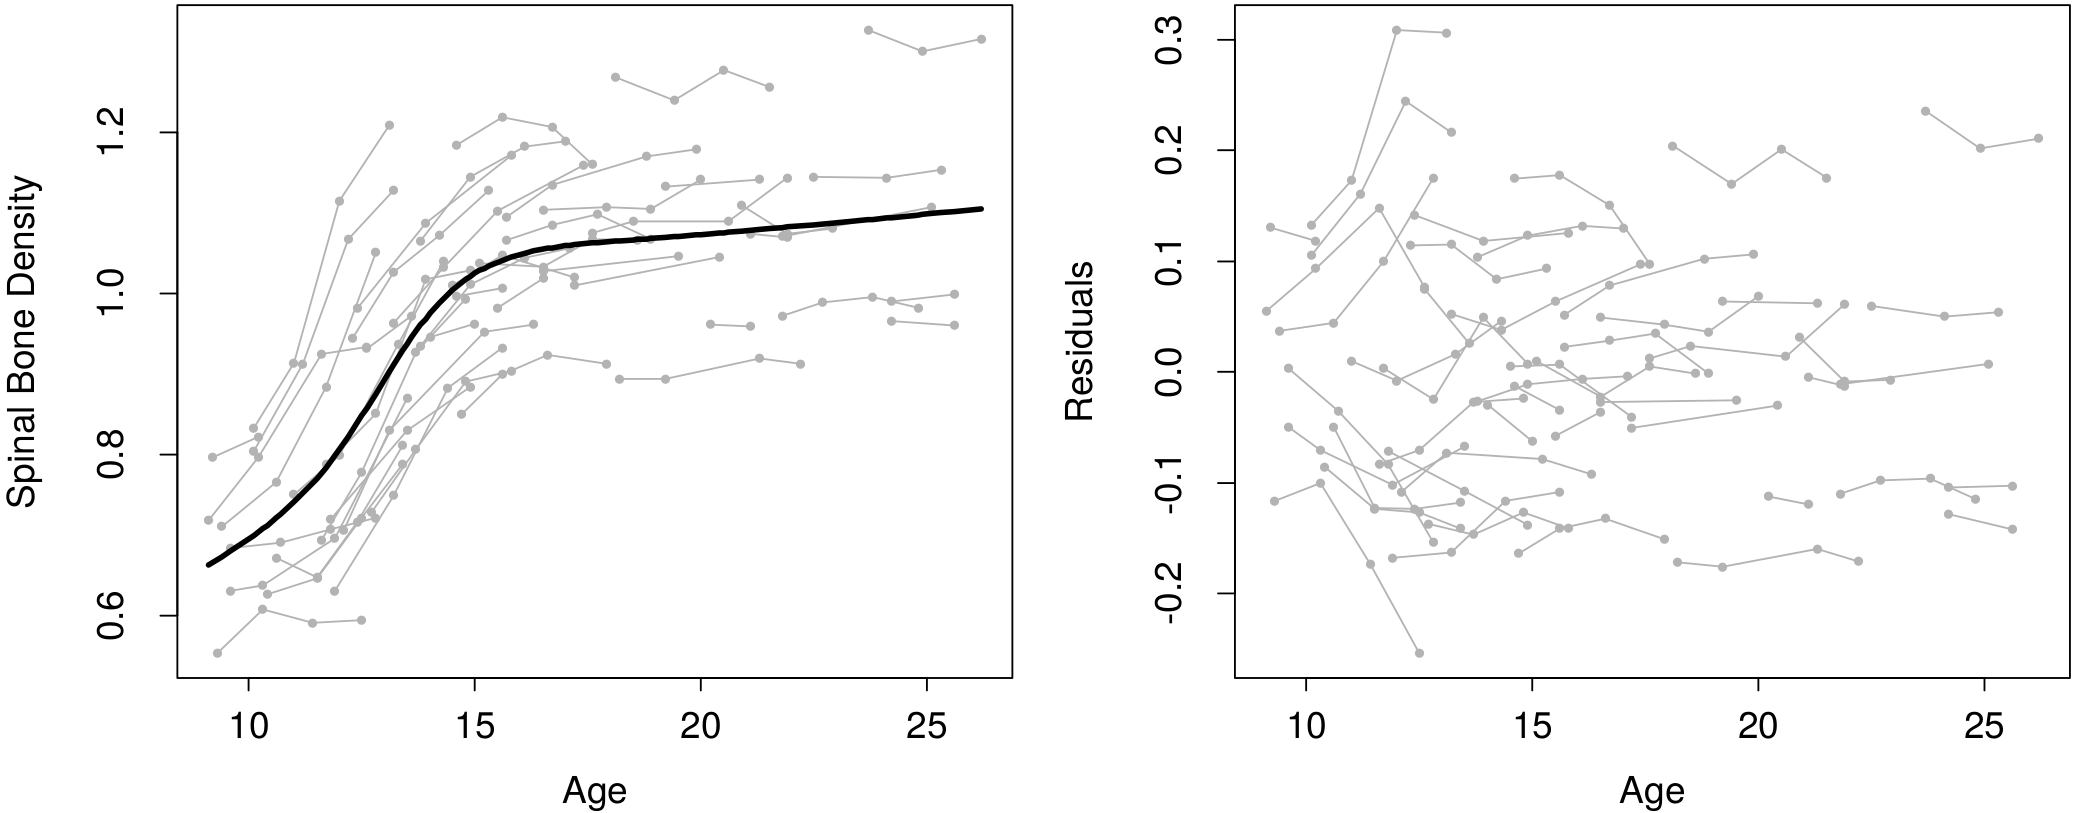
\includegraphics[width=\linewidth]{images/motivation}
  \caption{We observe gray fragments (individauls) and we want to recover the entire trajectories. [plots from \citet{james2000principal}]}
  \label{fig:motivation}
\end{figure}

We consider two cases:
\begin{itemize}
  \item We observe entire (noisy) processes and we want to recover the true processes,
  \item We observe the processes sparsely (Fig. \ref{fig:motivation}).
\end{itemize}

In both cases we assume that estimation of the mean process (thick line in Fig. \ref{fig:motivation}) is easy and we focus on second order properties (see \citet{rice1991estimating}).

\section{Notation}

For a diagonal matrix $D = \diag(d_1,...,d_p)$, define \[ D_\lambda = \diag((d_1 - \lambda)_+,(d_2 - \lambda)_+,...,(d_p - \lambda)_+) \] where $(x)_+ = \max(x, 0)$.

\section{Fully observed data}

In all models we will impose smooth structure by assuming that the true processes can be described in the basis $B = [b_1,b_2,...,b_p] \in \R^{d \times p}$, where $d \gg p$ and $b_1, b_2, ..., b_p$ are the first $p$ elements of some orthonormal basis of $\R^d$, i.e. $b_i \in \R^d$ and $b_i \perp b_j$ for $i \neq j$.

\subsection{Factor model (maximum likelihood)}

Let $\Theta \in \R^{p \times k}$ be $k$ factor loadings in the basis $(b_i)_{1 \leq i \leq p}$.


\begin{align}\label{eq:model}
  Y \sim \cN(0, B \Theta \Theta' B' + \sigma^2 I_d).
\end{align}
%where $\theta \in \R^{p}$ is a vector of coefficients of a population mean in the basis $B$. %, $\alpha_i \in \R^{1 \times k}$ such that $\alpha_i~\sim~\cN(0, D)$ is 'random effect' of subject $i$ with a diagonal $D \in \R^{k \times k}$ and $\varepsilon_i \sim \cN(0, \sigma I_d)$ is some observation noise.

We assume that $k < p$. Let
\begin{equation}
X = B'Y \sim \cN(\theta, \Theta \Theta' + \sigma^2 I_p).\label{model:x}
\end{equation}
Let $X_1,X_2,...,X_n$ be observations drawn from this distribution.
Let $S$ be the sample estimate of the covariance matrix of $X$. Let $S = V \Lambda V'$.
Theorem 9.4.1 in \citet{mardia1980multivariate} (after \citet{joreskog1967some}) states that for a fixed $\sigma$, the likelihood wrt. $(\Theta)$ is maximized by
\[
 \Theta = V\Lambda_{\sigma^2}^{1/2}.
\]
%where $\Lambda_{\sigma^2}$ is a diagonal matrix ``shrinked'' by $\sigma^2$, i.e. $\Lambda_{\sigma^2} = \diag(d_1,...,d_p)$, where $d_{i} = \max(\lambda_{i} - \sigma^2,0)$.
So the likelihood of $(\Theta,\sigma)$ can be parametrized by $\sigma$ and we find the solution analytically.

Two ways to estimate factor scores:

\paragraph{Bartlett's factor scores}
Bartlett's estimate of the scores is
\[
U' = (\Theta' \Psi^{-1} \Theta)^{-1} \Theta'\Psi^{-1} Y',
\]
where in our case $\Psi = \sigma^2 I$. thus
\begin{align*}
U' &= (\Theta' \sigma^{-2} I \Theta)^{-1} \Theta'\sigma^{-2} I Y'\\
&= (\Lambda_{\sigma^2}^{1/2}V' \sigma^{-2} V\Lambda_{\sigma^2}^{1/2})^{-1} \Lambda_{\sigma^2}^{1/2}V' \sigma^{-2} Y'\\
&= \sigma^{2}(\Lambda_{\sigma^2}^{1/2} \Lambda_{\sigma^2}^{1/2})^{-1} \Lambda_{\sigma^2}^{1/2}V' \sigma^{-2} Y'\\
&= (\Lambda_{\sigma^2})^{-1/2}V' Y'.
\end{align*}

Bartlett's factor score is unbiased.

\paragraph{Thompson's factor scores}
Thompson's estimate of the scores is
\[
U' = (I + \Theta' \Psi^{-1} \Theta)^{-1} \Theta'\Psi^{-1} Y',
\]
which gives
\begin{align*}
U' &= (I + \Lambda_{\sigma^2})^{-1} \Lambda_{\sigma^2}^{1/2}V' Y'
\end{align*}

It gives more accurate predictions \citet{paterek2007improving}.

\citet{krzanowski1995multivariate} and \citet{tipping1999probabilistic} show that
\[
\sigma_{ML}^2 = \frac{1}{p-q} \sum_{i = p-q+1}^d\lambda_i.
\]
Other references: \citet{rubin1982algorithms}.



\subsection{Factor analysis (PC)}

We initially 'guess' an estimator for $\sigma$, say $\hat\sigma_1$ in \eqref{model:x}. We decompose $S~-~\hat\sigma_1^2I_d~=~\hat\Theta_1 \hat\Theta_1'$. We estimate $\sigma$ and estimate $\hat\Theta_2$. We iterate and converge to $\hat\Theta$. See \citet{lawley1971factor}.

\subsection{Factor analysis (centroid method)}
 \citet{lawley1971factor}

%\subsection{Tresholded SVD}
%Let $X_1,X_2,...,X_n$ be observations from \eqref{model:x}. Let $\bX = [X_1',X_2',...,X_n']'$. Consider



%% \section{Sparsly observed data}

%% \subsection{Sparse functional PCA}
%% Likelihood of $Y_i$ can be written as
%% \[
%% Y_i \sim \cN(0, \sigma^2 I_d + B \Theta D \Theta' B').
%% \]
%% Our goal is to find $\theta, \Theta, D$ maximizing
%% \[
%% \prod_{i=1}^N \frac{1}{(2\pi)^{d/2} |\sigma^2I_d + B \Theta D \Theta' B'|^{1/2}} \exp\left\{ -(Y_i)'(\sigma^2 I_d + B \Theta D \Theta'B' )^{-1} (Y_i) / 2\right\}.
%% \]
%% Assume $\alpha_i$ are known. Then the likelihood is
%% \[
%% \prod_{i=1}^N \frac{1}{(2\pi)^{d/2} \sigma^d |D|^{1/2}} \exp\left\{ -(Y_i - \alpha_i\Theta B)'(Y_i - \alpha_i\Theta B) / 2\sigma^2 - \frac{1}{2}\alpha_i' D^{-1} \alpha_i \right\}.
%% \]
%% Maxmizing this expression is equivalent (TODO: check) to minimizing
%% \begin{align*}
%% \sum_{i=1}^N \left\{ (Y_i - \alpha_i\Theta B)'(Y_i - \alpha_i\Theta B) + \sigma^2 \sum_{j=1}^k \frac{\alpha_{i,j}^2}{D_{jj}}\right\} =&\\
%% \sum_{i=1}^N \| Y_i - \alpha_i\Theta B\|^2 + \sigma^2 \sum_{j=1}^k \frac{1}{D_{jj}}\sum_{i=1}^N\alpha_{i,j}^2 =&\\
%% \| Y - A\Theta B\|_F^2 + \sigma^2 \| A D^{-1/2} \|_F^2,
%% \end{align*}
%% where $A = [\alpha_1,\alpha_2,...,\alpha_N]'$.
%% Thus, the algorithm solves
%% \begin{align}\label{eq:optpca}
%% \argmin_{\theta,A,\Theta}\| Y B' - A\Theta\|_F^2 + \sigma^2 \| A D^{-1/2} \|_F^2.
%% \end{align}

\subsection{Regularized SVD}
Given $N$ observations from \eqref{eq:model}, let
\[
Y =  X\Theta B + \varepsilon.
\]
Consider the optimization problem
%% \usepackage{graphicx}
%% \[
%% \argmin_{\theta, A, \Theta} \| Y - (\mathbf{1}\theta B + A \Theta B)\|_F^2.
%% \]
%% Since $B$ is orthonormal, the problem is equivalent to 
%% \[
%% \argmin_{\theta, A, \Theta} \| YB' - (\mathbf{1}\theta + A \Theta)\|_F^2. 
%% \]
%% The solution is given by the reduced-rank SVD of $YB'$. We get $U,V$ such that
%% \[
%% \mathbf{1}\theta + A \Theta = UV'.
%% \]
%% We can decompose it to 
%% \[
%% \theta = U_0V' \text{ and } \Theta = U_1 V',
%% \]
%% where $U_0$ is the mean of rows of $U$ and $U_1 = U - \mathbf{1}U_0$.
%% Now, suppose we don't know the rank of $A$ and we want to find a reduced-rank solution. We add the penalty term
%% \[
%% \argmin_{\theta, A, \Theta} \| YB' - (\mathbf{1}\theta + A \Theta)\|_F^2 + \lambda\|\mathbf{1}\theta + A \Theta\|_*
%% \]
%% which is equivalent to
\begin{align}\label{eq:optsvd}
\argmin_{W} \frac{1}{2} \| YB' - W \|_F^2 + \lambda\|W\|_*.
\end{align}
%% and again reduced-rank SVD gives solutions for different ranks depending on $\lambda$.
%% Note that
%% \[
%% \|A\|_* = \sum_{i = 1}^k s_i = \| A D^{-1/2} \|_F^2,
%% \]
%% so the solutions \eqref{eq:optpca} and \eqref{eq:optsvd} should be (roughly) equivalent as long as $\lambda = \sigma^2$.
\citet{cai2010singular} show that the solution of \eqref{eq:optsvd} is given by a shrinked SVD $W = UD_\lambda V'$.

\subsection{Simulation}

We take the grid of size $d = 51$ and a spline basis of $9$ functions (Figure \ref{fig:basis}. We generate observations from model $\eqref{eq:model}$ with $k = 9$ true components. We set $\Theta\Theta'$ to be a matrix with eigenvalues $\diag[1,0.9,0.5,e^{-3},...,e^{-8}]$. We observed values with uncorrelated gaussian noise with $\sigma^2 = 0.25$. The matrix is fully-observed.

\begin{figure}[h]
  \includegraphics[width=\linewidth]{images/simulation-basis}
  \caption{Basis on the grid $G$ of $d=51$ equidistributed points and its othronormalized equivalent.}
  \label{fig:basis}
\end{figure}

In functional PCA we run the procedure with different $K = 1,2,...,9$ and in Soft-Impute we run the estimation procedure with different $\lambda$. We present the best results in Figure \ref{fig:results}. We analyze two errors: mean squared distance (1) from the observed points ($M_O$) and (2) from the true processes ($M_T$). For now, no cross-validation -- only in-sample fit.

Preliminary results are presented in (Table \ref{tab:results}).
\begin{table}[h]
  \centering
\begin{tabular}{lcc}
                  & $M_O$ & $M_T$\\
\hline
Soft-Impute  & 0.91 (sd=0.006) & 0.97 (sd=0.07)\\ 
Sparse fPCA & 0.93 (sd=0.009) & 0.91 (sd=0.07)\\
\end{tabular}
  \caption{Results from only ten trials (TODO).}\label{tab:results}
\end{table}

Results from one of the simulations are presented in Figure \ref{fig:results}. In Figure \ref{fig:components} we plot components and in Figure \ref{fig:scores} we plot scores.

\begin{figure}[h]
  \includegraphics[width=\linewidth]{images/simulation-results}
  \caption{5 example curves. True processes (top-left), Observed processes (top-right). Soft-impute estimates (bottom-left) and sparse functional PCA estimates (bottom-right).}
  \label{fig:results}
\end{figure}

\begin{figure}[h]
  \includegraphics[width=\linewidth]{images/simulation-components}
  \caption{Components}
  \label{fig:components}
\end{figure}

\begin{figure}[h]
  \includegraphics[width=\linewidth]{images/simulation-scores}
  \caption{Scores}
  \label{fig:scores}
\end{figure}

\bibliography{report}

\end{document}
